\documentclass[12pt]{article}

\usepackage[pdftex]{graphicx}
\usepackage{cancel}
\usepackage[margin=4cm]{geometry}
\usepackage[hidelinks]{hyperref}
\usepackage{fancyhdr}
\usepackage{amsmath}
\usepackage{amsfonts}

\newcommand\tab[1][1cm]{\hspace*{#1}}
\newcommand{\HRule}{\rule{\linewidth}{0.5mm}}
\newcommand{\course}{COMS 474}

\setcounter{secnumdepth}{0} % Disable section/subsection numbering
\hyphenpenalty 10000 % Prevent words from being broken over multiple lines
\exhyphenpenalty 10000 % Prevent words from being broken over multiple lines

% Margins
\topmargin=-0.45in
\evensidemargin=0in
\oddsidemargin=0in
\textwidth=6.5in
\textheight=9.0in
\headsep=0.25in
\title{ \course \\\large Homework 4 }
\author{ Haadi Majeed }
\date{Spring 2022}


\pagestyle{fancy}
\fancyhead{}
\fancyfoot{}
\lhead{\course}
\chead{Haadi Majeed}
\rhead{Page \thepage}

\begin{document}
\maketitle
\pagebreak

% Optional TOC
%\tableofcontents
\pagebreak
\section{Problem 1}
 [24 points total (5,5,3,3,4,4)]\\
Suppose you use lasso fit to a linear model for a data set. Let $\beta^*(\lambda)$ denote the lasso solution for a specific $\lambda$ (i.e. the coeffcient vector you get for that $\lambda$).
\\\\Provide explanations for your answers to the following questions.

\subsection{Part A}
Describe how the \underline{training} MSE changes as a function of $\lambda$, including $\lambda = 0$ and as $\lambda \rightarrow \infty$\\\\
The training MSE of the function $\beta^*(\lambda)$ would return the least squares fit when $\lambda = 0$. The value output does change though as $\lambda$ grows in size, with the upper bound of $\infty$ being the most ideal constant that could be supplied to the equation, this is because at \emph{some} point, $\lambda$ will hit the absolute minimium of the function, which would be within the range of $0\rightarrow\infty$.

\subsection{Part B}
Describe how the \underline{hold-out} MSE changes as a function of $\lambda$, including $\lambda = 0$ and as $\lambda \rightarrow \infty$\\\\
The hold-out MSE \emph{should} look similar to the training MSE and by applying a similar set of logic, the models should look relatively the same as it is from the same overall set of data. The resulting model should have an absolute minimium which would indicate what the most ideal $\lambda$ would be. This value should be, if not exactly, then very close to where the training set's absolute minimium should be at. The image I have attached below is from the notes and displays what the models could look like as an example.
\begin{center}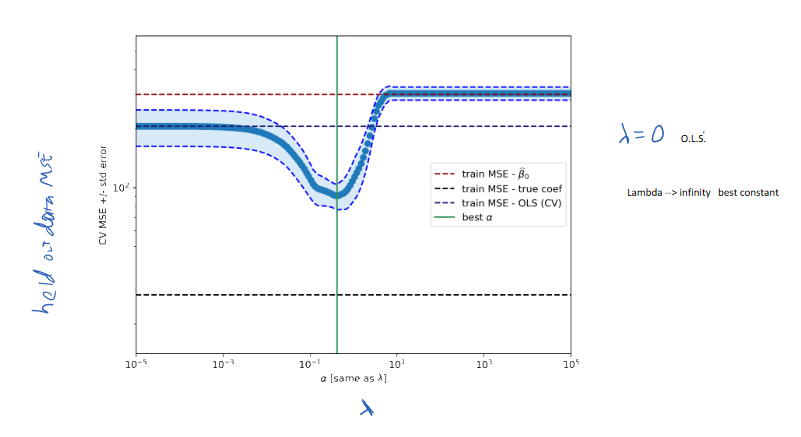
\includegraphics[width=1\textwidth]{p1.b.png}\end{center}

\subsection{Part C}
Describe $\beta^*(0)$.\\\\
When initially at $\beta^*(0)$, the function's value that it would return would simply be the L.S.F (least squares fit) value.

\subsection{Part D}
Describe what happens to $\beta^*(0)$ as $\lambda$ grows.\\\\
The model $\beta^*(0)$ would cover every possible value between $0\rightarrow\infty$ and would eventually hit the functions aboslute minimium in a concave region. This is where it deviates off the null model and no longer just returns zero, and insteal will indicate what the absolute minimium, or the most ideal $\lambda$, would be.

\subsection{Part E}
If you used ridge regression instead of lasso, explain how your answers to (a).-(d). would differ. \\\\
If we were to use ridge regression, we should expect a bit of variance in the data since they approach model slightly differently. Another attribute of ridge regression is that it is not capable to have sharp points in the model, thus intersections at an axis is not common. This subsequently results in non-zero estimations. The models generated by this when comparing the training vs the hold-out data should look very similar to each other due to data distribution. Ridge regression looks at both extremes and steps through the function looking at each step from $0\rightarrow\infty$. It also penalises $\lambda\rightarrow\infty$ signifigantly more than it would $\lambda = 0$. When$\lambda = 0$ it would return the Least Squares estimation, while when $\lambda\rightarrow\infty$ it estimates the model will approach zero and the shrinkage penalty grows.

\subsection{Part F}
We discussed the “constrained form” of lasso, with a constraint of the form
\begin{center}
    \[\sum_{i=1}^{p}|\beta_j| \leq t\]
\end{center}
Which value, or limiting value, of $t$ coresponds to $\lambda = 0$ and which corresponds to $\lambda \rightarrow \infty$\\\\
The value of $t$ would equate to $|\beta_1|^1 + |\beta_2|^1$ since $t$ represents $\lambda$ but in a constrained environment instead. The point at which the red oval from figure 6.7 from the book (attached below)
\begin{center}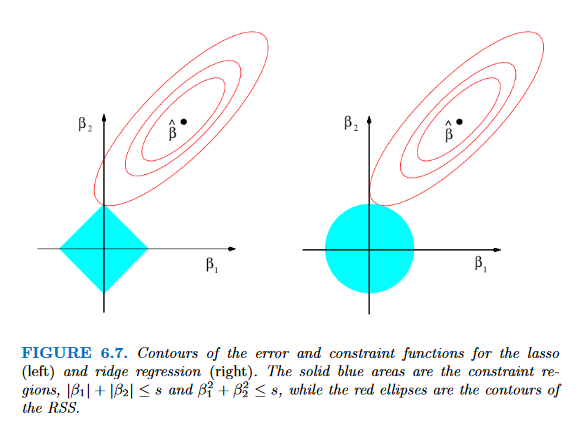
\includegraphics{p1.f.png}\end{center}
Should $\lambda = 0$ then $t = |\beta_1|^1 + |\beta_2|^1$ since we are restricted by $\sum_{j=1}^p |\beta_j|$ having to be within the bound set by $t$ and the expected output would quite small. For when $\lambda\rightarrow\infty$, then $t = 0$ since the solution of the Least Squares Fit since it would be encompassed by the range set by $t$.



\pagebreak
\section{Problem 2}
 [15 points]\\
You have already seen formulas for the best intercept in linear models when there are no
features $p = 0$ and a single feature $p = 1$. You will now look at what happens with $p$ features
when we center the data.\\
Recall that “centering” a feature means subtracting its mean. For example, if the sample values
for feature $X_4$ are $\begin{bmatrix} 5 \\0\\1\end{bmatrix}$, which has a mean of $2$, \\we could replace it with $\begin{bmatrix} 5 - 2\\0 - 2\\1 - 2\end{bmatrix} = \begin{bmatrix} 3\\-2\\-1\end{bmatrix}$ which has a mean of $0$. Thus if feature $X_4$ is centred, then $\sum^n_{i=1}X_4(i) = 0$.\\\\

What is the value of the intercept $\beta^*_0$ in the ordinary least squares solution, i.e.
\begin{center}
    \[
        (\beta^*_0, \beta^*_1, \dots, \beta^*_p) = \underset{(\beta^*_0, \beta^*_1, \dots, \beta^*_p)\epsilon\mathbb{R}^{p+1}}{\text{arg min}}\frac{1}{n}\sum_{i = 1}^{n} \bigg( Y(i) - \beta_0 \sum_{j=1}^p\beta_jX_j(i)\bigg) ^2
    \]
\end{center}
when the features ${X_1, \dots, X_p}$ are all centered? (e.g. $\sum_{i=1}^nX_j(i) = 0$ for $ j = 1, \dots, p$). (You do not need to use a second derivative test or solve for \{$\beta_1^*, \dots, \beta_p^*$\}, just use the first derivative test $0 = \frac{\partial}{\partial\beta_0}$ MSE).

%--/Paper--

\end{document}